\documentclass[11pt]{article}
\usepackage[margin=1in]{geometry}
\usepackage{hyperref}
\usepackage{graphicx}
\usepackage{float}
\usepackage[style=ieee]{biblatex}

\title{Related News Injection via HTTPS Proxy}
\author{Kyle Wigdor and Yeju Suh}
\date{}

\addbibresource{refs.bib}

\begin{document}
\maketitle

\section{Introduction}
Journalism is intended to inform the public and provide the context necessary for individuals to form their own opinions. However, modern online news consumption is increasingly shaped by recommendation algorithms and link-following that prioritizes content from the same outlet or from ideologically similar sources. As a result, readers are exposed to reinforcing perspectives rather than independent reporting \cite{bias}. To address this, we propose a man-in-the-middle (MITM) proxy that injects related coverage from independent sources directly into online news websites\footnote{Code available at \url{https://github.com/nvdaz/related-news/tree/main}}. Rather than relying on a single outlet's framing, users are presented with diverse reporting on the same event along with highlights of key areas of agreement and disagreement, promoting a more comprehensive and balanced understanding of the news.

\section{System Design}

\subsection{Proxy Layer}
The MITM proxy is implemented using Goproxy \cite{goproxy} and a custom Certificate Authority (CA) to enable TLS interception, allowing the system to inspect and modify encrypted traffic. For HTML responses, the proxy injects a short script that loads the frontend, while all non-HTML content is left untouched. The proxy is also responsible for routing the client to the frontend and backend services.

\subsection{Frontend Overlay}
The frontend, shown in Figure~\ref{fig:design}, is built with React \cite{react} delivered as a JavaScript bundle that runs after the host page loads and sends the page content to the backend for analysis and source retrieval. This happens asynchronously, so users can continue using the page uninterrupted. Results appear in a pop-up panel showing recommended sources with brief summaries and highlighted agreements and disagreements. Users can like or dislike sources, which influences future recommendations.

\subsection{Backend Service}
FastAPI \cite{fastapi} is used to serve the backend, which uses a multi-stage pipeline of retrieval and synthesis to develop a list of related sources. In the retrieval stage, Gemini \cite{google_gemini} with the Google Search tool is used to identify relevant news articles and generate brief preliminary summaries. To ensure found URLs are valid, they are sourced from the grounding context instead of LLM output. In the synthesis stage, each source is further analyzed by Gemini to produce refined summaries, as well as structured points of agreement and contention across sources. These results are then returned to the frontend for presentation to the user.

\section{Evaluation}

\subsection{Page Load Overhead}
Figure~\ref{fig:proxyperfeval} shows the performance overhead introduced by the MITM proxy and script injection. All experiments were conducted using the Firefox web browser \cite{firefox}. Load times varied substantially across websites, with pages requiring on average 178.68\% of their original, unproxied time to reach the \texttt{DOMContentLoaded} event, which measures the time to load all HTML elements \cite{mdn_domcontentloaded}. This overhead is primarily caused by TLS termination at the proxy and the buffering required to modify response bodies before they are forwarded to the client.

Pop-ups were generated asynchronously via LLM-based retrieval and search performed by the backend service without delaying page load times. Generation time varied across sites, with pop-ups taking an average of 28.70 seconds to create; detailed results are shown in Figure~\ref{fig:llmperfeval}.

\subsection{LLM Performance}
On long-form, subjective news articles, the assistant was able to surface relevant perspectives from outlets with differing editorial positions. The generated cross-references effectively highlighted points of agreement and disagreement across sources, helping readers contextualize the coverage. Performance degraded as the available text decreased. For news stories delivered primarily through video, the assistant was limited to captions, which reduced the depth and specificity of its references. On news aggregators, the layout containing varied stories further constrained the system, leading to more generic and less targeted cross-references.

The worst-case behavior emerged on pages that were not news content at all, where the injection was enabled for exploratory purposes. In these settings, the assistant typically produced loosely related news items whose cross-references were largely irrelevant to the page itself and often provided little to no analytical value.

\section{Reflection}
Ensuring that the LLM-based search did not hallucinate sources was the most technically challenging part of the project. Without tools, LLMs routinely hallucinated URLs, and even with search support they often failed to reliably link source URLs to generated text. To solve this, we used Gemini with the Google Search tool because it provides grounding annotations that explicitly tie each text segment to a real source URL. These annotations were parsed to build a set of verified URLs, which were then passed into later LLM calls to refine each source and its context into displayable elements.

With additional development time, broader support for diverse website types would be useful. While the current design works well for typical long-form news articles, other content formats would benefit from different presentations. For example, news aggregators could provide source lists on a per-article basis rather than for the entire page, or even to annotate individual headlines as controversial when there are many sources with differing perspectives. Furthermore, more effort could have been spent optimizing LLM prompts for quality and latency.

The delivery mechanism for the injection could also be improved. Goproxy was selected for its simplicity, but a production deployment would more likely use a high-performance proxy such as Envoy \cite{envoy} or Squid \cite{squid}. Alternatively, the injection could be delivered via a browser extension \cite{webextensions} rather than a network-level proxy, which would reduce latency and improve security by eliminating the need for MITM interception with a local CA.

\newpage
\printbibliography

\newpage
\appendix

\section{Design}
\begin{figure}[H]
  \centering
  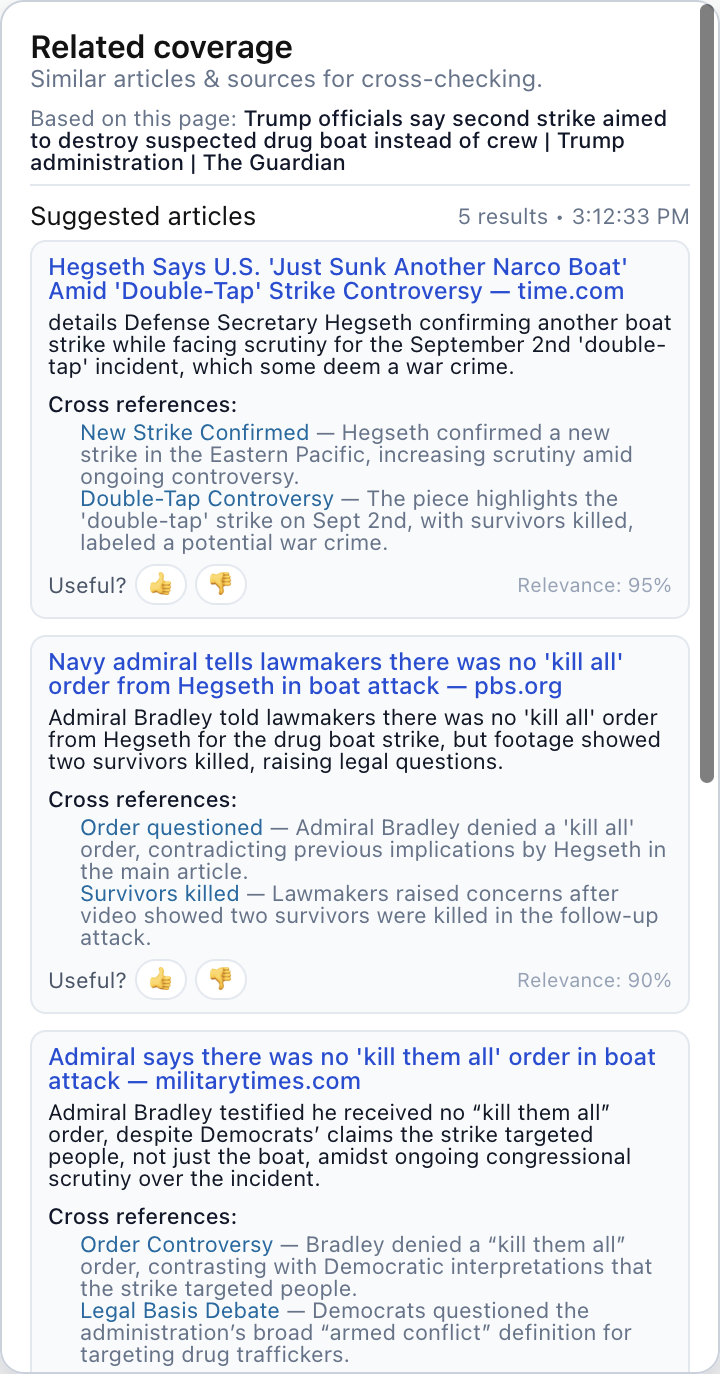
\includegraphics[width=0.5\textwidth]{example.png}
\caption{Design of the pop-up screen on The Guardian (source: \url{https://www.theguardian.com/us-news/2025/dec/03/trump-officials-boat-strikes-legal-analysis}, identified by querying ChatGPT for a recent article on a controversial topic).  The subtitle displays the title of the currently viewed article, while the number of related articles found and the time of the search are shown above. The related articles are presented as a vertical series of cards, each featuring a clickable headline. Each card also includes a brief summary and cross-references indicating whether the articles corroborate or challenge one another.}
  \label{fig:design}
\end{figure}


\section{Proxy Performance Overhead}
\begin{figure}[H]
    \centering
    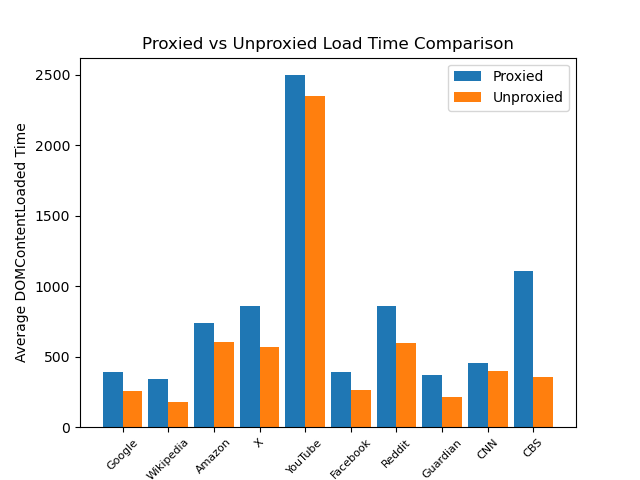
\includegraphics[width=\textwidth]{graph/eval.png}
    \caption{Performance evaluation of proxied versus unproxied connections measured by \texttt{DOMContentLoaded} time averaged over three trials. Overhead increases observed across major sites include Google (151.88\%), Wikipedia (196.58\%), Amazon (122.96\%), X (150.15\%), YouTube (106.24\%), Facebook (146.92\%), Reddit (142.94\%), The Guardian (174.61\%), CNN (113.57\%), and CBS (312.46\%). On average, a 161.83\% overhead was observed.}
    \label{fig:proxyperfeval}
\end{figure}

\section{LLM Performance}
\begin{figure}[H]
    \centering
    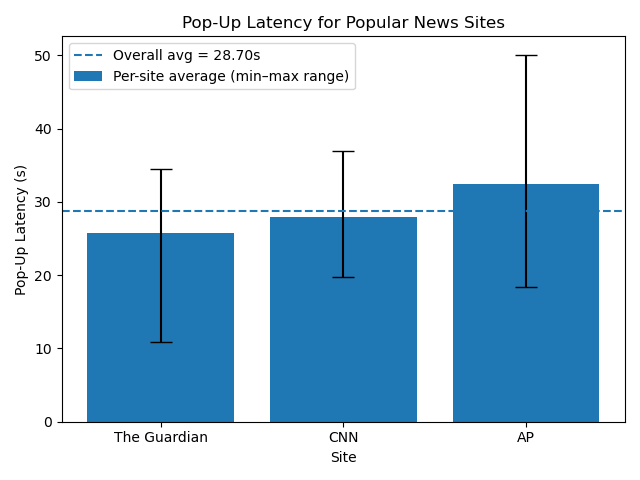
\includegraphics[width=\textwidth]{graph/llm.png}
    \caption{Pop-up latency evaluation across major news sites measured in seconds. The Guardian exhibited an average latency of 25.74\,s (min: 10.87\,s, max: 34.56\,s), CNN showed an average of 27.95\,s (min: 19.80\,s, max: 36.89\,s), and AP recorded the highest average latency at 32.42\,s (min: 18.44\,s, max: 50.10\,s). The overall average latency across all measurements was 28.70\,s.}
    \label{fig:llmperfeval}
\end{figure}



\end{document}
